\documentclass{sciposter}
\usepackage{lipsum}
\usepackage{epsfig}
\usepackage{tikz}
\usepackage{amsmath}
\usepackage{amssymb}
\usepackage{multicol}
\usepackage{graphicx,url}
\usepackage[portuges, brazil]{babel}   
\usepackage[utf8]{inputenc}
\usepackage{fancybox}
\usepackage{xcolor}

\newtheorem{Def}{Definição}

\title{Modelo de Consulta de Finanças III}
% Título do projeto

\institute 
{Bacharelado em Economia\\
Insper - Instituto de Ensino e Pesquisa\\
São Paulo, Brasil}
% Nome e endereço da Instituição

\rightlogo[1]{logo-insper.png}  % Substitua pelo logo do Insper

\begin{document}

\conference{{\bf Finanças III}, Curso de Economia - Insper, 2024, São Paulo, Brasil}

\maketitle

%%% Início do ambiente Multicolunas
\begin{multicols}{3}

%%% Resumo
\begin{abstract}
Este documento fornece um modelo de consulta para a disciplina Finanças III. Ele organiza os principais conceitos e tópicos relevantes para facilitar a revisão do curso.
\end{abstract}

%%% Introdução
\section{\textbf{Revisão de Valuation}}
\subsection{\textbf{Explicar como uma empresa nascente financia sua operação}}
\subsubsection*{\textbf{Estágios de Vida da Empresa e Taxa de Crescimento}}
\begin{figure}[H]
    \centering
    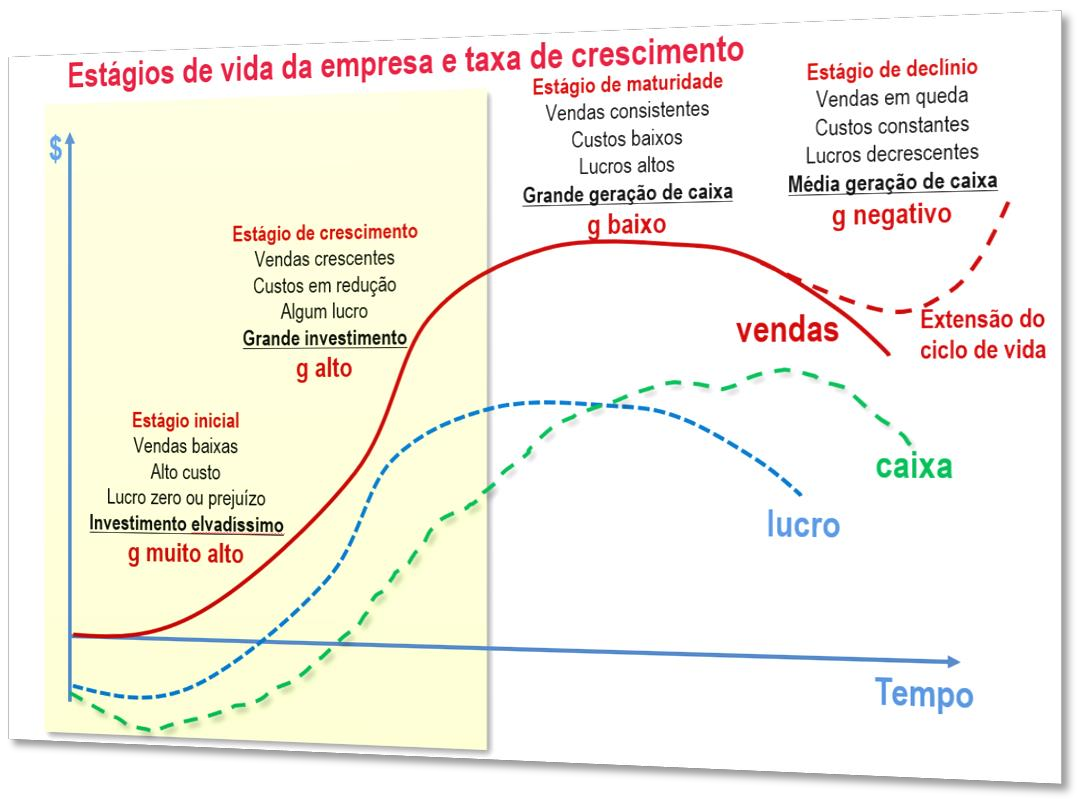
\includegraphics[width=1.0\textwidth]{evetc.png}
\end{figure}
\subsubsection*{\textbf{Financiadores Típicos para Empresas desde Estágios Iniciais}}
\begin{itemize}
    \item Startups\begin{itemize}
        \item Sócios Fundadores (FFF) Funders, Family and Fools
        \item Investidores-Anjo(Angels)
        \item Ventury Capital Funds (VCs)
        \item Private Equity Funds (PEs)
        \item IPO - Sociedade Anônima
        \item Emissão de Títulos e Emprestímos
    \end{itemize}
    \item Empresas Pequenas e Médias \begin{itemize}
        \item Sócios Fundadores
        \item Sociedade Anônimas
        \item Empréstimos
    \end{itemize}
\end{itemize}

\subsubsection*{\textbf{Detalhamento das Fases Inicias}}
\begin{itemize}
    \item Pre-Seed \begin{itemize}
        \item Ideia e equipe funcionam?
        \item Validação do negócio e MVP (viabilidade mínima do produto)
        \item FFF, anjos e aceleradores
        \item Até US\$ 200 mil
        \end{itemize}
    \item Seed \begin{itemize}
        \item Dá para escalar ?
        \item Investimento em vendas, marketing e operações
        \item Anjos, fundos seed e micro-VC
        \item US\$ 300 mil a 700 mil
        \end{itemize}
    \item Seria A \begin{itemize}
        \item Dá para escalar rápido ?
        \item Estruturação da Empresa
        \item Fundos VC, dividas ou equity
        \item US\$ 1 a 5 milhões
        \end{itemize}
    \item Series B, C etc \begin{itemize}
        \item Dá para consolidar 
        \item Ganho de mercado, geração de caixa, aquisição de empresas, internacionalização
        \item Fundos VC, dívidas ou equity
        \item Em geral na faixa de US\$ 50 a 250 milhões
        \end{itemize}
    \item Saídas : IPO, Investidor Estatégico, etc 
\end{itemize}

\subsubsection*{\textbf{Avaliação de startups e projetos novos}}
\begin{figure}[H]
    \centering
    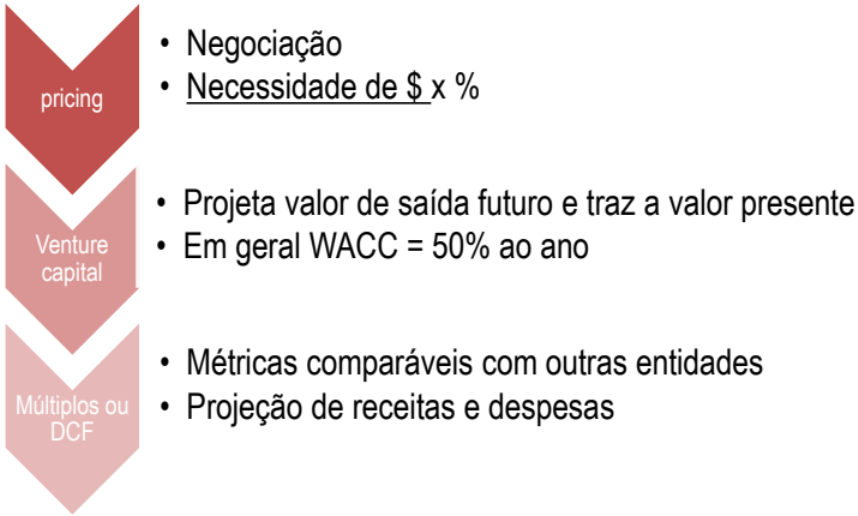
\includegraphics[width=1.0\textwidth]{aspn.png}
\end{figure}

\subsubsection*{\textbf{Pre-money e post-money}}

\begin{tikzpicture}
    \node[draw, fill=red!70, text width=3cm, text centered, rectangle] (postmoney) at (0,0) {Valor\\ Post\\ money};
    
    \node[text centered, text width=1cm] (equals) at (3,0) {\Huge $=$};
    
    \node[draw, fill=green!60, text width=3cm, text centered, rectangle] (premoney) at (6,0) {Valor\\ Pre-money};
    
    \node[text centered, minimum size=1cm] (plus) at (9,0) {\Huge $+$};
    
    \node[draw, fill=purple!60, text width=4cm, text centered, rectangle] (dinheiro) at (12.5,0) {Dinheiro\\ recebido na\\ rodada (aporte)};

\end{tikzpicture}

\textbf{Passo a Passo}

\begin{figure}[H]
    \centering
    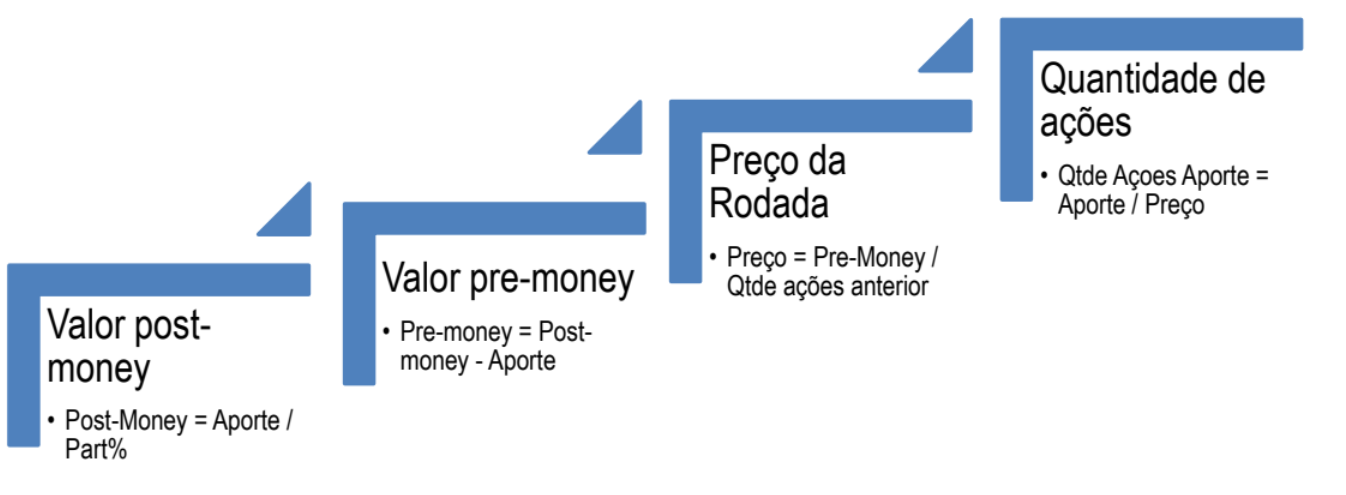
\includegraphics[width=0.75\textwidth]{preposmoney.png}
\end{figure}

\subsection{\textbf{Explicar como uma empresa nascente toma decisões de investimento}}
\subsubsection*{\textbf{Como uma startup deveria tomar uma decisão de investimento}}
\begin{itemize}
    \item Oportunidade de Mercado 
    \item Impacto na Empresa 
    \item Estratégia de Crescimento
    \item Retorno do Investimento \begin{itemize}
        \item Aqui os investidores novos pensam na estratégia de saída e raramente no fluxo de caixa
        \item Fundador pensam mais na estratégia da empresa longo prazo
    \end{itemize}
    \item Risco
    \item Recursos
\end{itemize}

\subsubsection*{\textbf{Quais critérios são usados pelo VCs}}
Um estudo de Havard identifica as métricas mais populares usadas, apesar de que nenhuma métrica é adequada para valiar incertezas extremas, um desafio central no empreendimento.

\begin{itemize}
    \item Multiple on Invested Capital (MOIC) \begin{itemize}
        \item $\textbf{MOIC} = \frac{Valor \ da \ Empresa }{Capital \ Investido}$
    \end{itemize}
    \item TIR (do valor de saída em relação ao aporto) \begin{itemize}
        \item \textbf{TIR} : $\sum_{t=0}^{N}\frac{CF_t}{(1+TIR)^t}=0$
    \end{itemize}
\end{itemize}


\subsubsection*{\textbf{Método sofisticado utilizando árvore de decisão gerenciais}}

\begin{figure}[H]
    \centering
    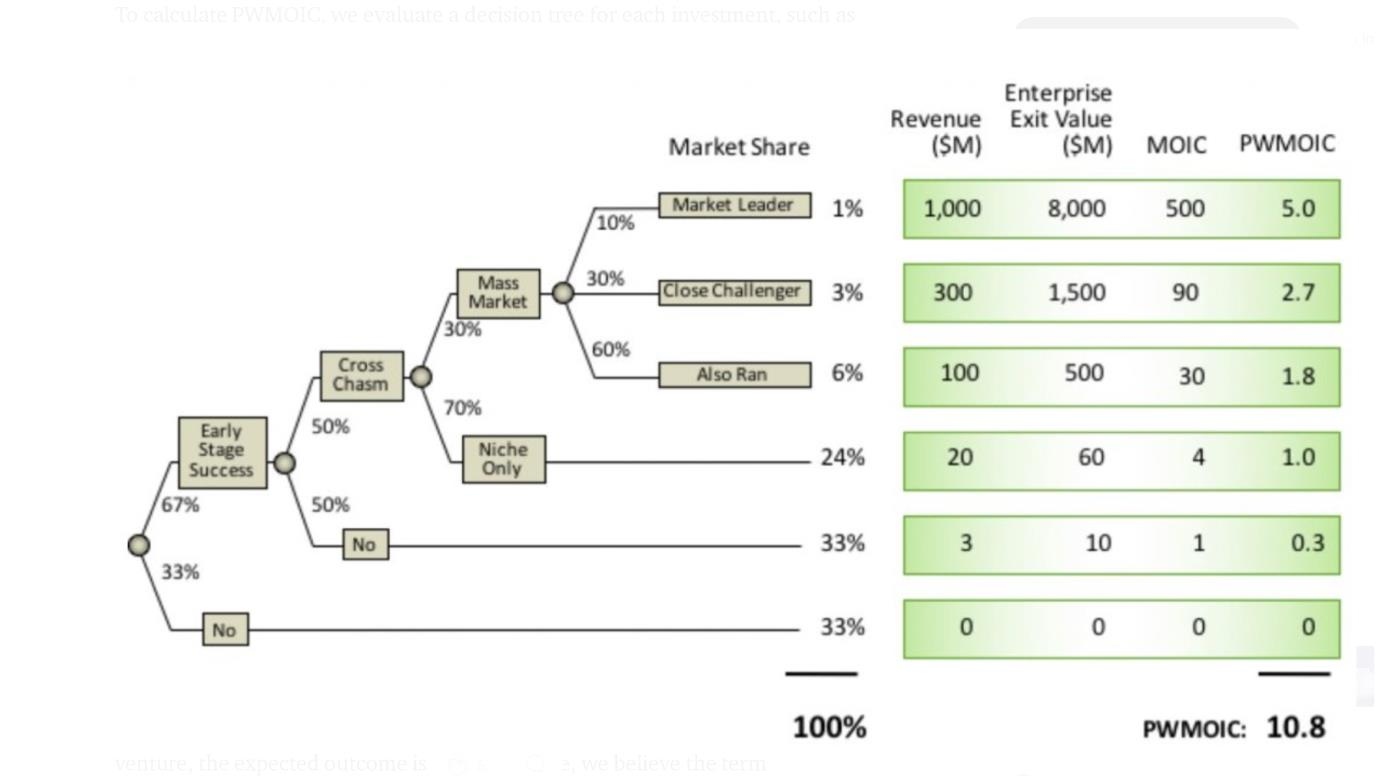
\includegraphics[width=0.75\textwidth]{arvore.png}
\end{figure}

\subsection{\textbf{Identificar os principais indicadores utilizados por startups para analisar seu desempenho financeiro}}

\subsubsection*{\textbf{Princiapais Indicadores usados por Startups}}
\textbf{Indicadores de retorno por cliente} \begin{itemize}
    \item Como é difícil saber quantos clientes, fica mais fácil analisar um cliente incremental
    \item \textbf{CAC (Custo de Aquisição de Cliente)} : É o valor que uma empresa gasta para adquirir um novo cliente. Este número é importante porque ajuda a entender se a empresa está investindo mais do que está ganhando com novos clientes.
    \item \textbf{LTV (Life Time Value): É o valor que um cliente é esperado para gerar ao longo do tempo. Este número é importante porque permite que a empresa entenda se o CAC está alinhado ao valor que o cliente está gerando.} \begin{itemize}
        \item \textbf{Ticket Médio} : É o valor médio que um cliente gasta em cada transação. Este número é importante porque indica se a empresa está vendendo produtos ou serviços de alto valor.
    \end{itemize}
\end{itemize}

\subsection{\textbf{Explicar os métodos mais comuns de avaliar uma startup}}
\subsection{\textbf{Calcular o valor de uma startup por meio de métodos mais usados atualmente}}
\subsubsection{\textbf{Métodos de Múltiplos}}
\subsubsection{\textbf{Métodos de Fluxo de Caixa Descontado}}
\subsubsection{\textbf{Método de Venture Capital}}
\subsection{\textbf{Explicar como os métodos de fluxo de caixa descontado podem ser aplicados em empresas reais no Brasil}}

\section{Opções - Conceitos}
    \begin{center}
    Comprador = Titular / Long
    
    Vendedor = Lançador / Short
    \end{center}
\vspace{0.75 cm}
\subsection*{\textbf{Agentes de mercado}}
\begin{itemize}
    \item \textbf{Hedgers:} Proteção contra riscos
\end{itemize}
\begin{itemize}
    \item \textbf{Especuladores:} Alavancagem da exposição ao ativo objeto
    \item \textbf{Arbitradores:} Ganhos "garantidos" sem risco
\end{itemize}

\vspace{0.75 cm}
\subsection*{Elementos que caracterizam uma opção}
\begin{itemize}
    \item \textbf{Ativo objeto} (ação, moeda, commodity, taxa de juros, etc)
    \item \textbf{Strike} (preço de exercício)
    \item \textbf{Data de vencimento}
    \item \textbf{Preço de negociação} (Prêmio)
\end{itemize}

\vspace{0.75 cm}
\subsection*{\textbf{Tipos de opção}}
\begin{itemize}
    \item \textbf{Européia:} exercício apenas no vencimento
\end{itemize}
\begin{itemize}
    \item \textbf{Americana:} exercício à critério do comprador
\end{itemize}

\vspace{0.75 cm}
\subsection*{\textbf{Nomenclatura com relação ao strike (calls)}}
    \begin{itemize}
        \item \textbf{ITM:} preço do ativo maior do que o strike
        \item \textbf{ATM:} preço do ativo igual ao strike
        \item \textbf{OTM:} preço do ativo menor do que o strike
    \end{itemize}
\textbf{Obs:} Iverter o racioncínio para puts
\item \vspace{0.75 cm}

\subsection*{\textbf{Valor intrínseco e temporal}}
    \begin{center}
    Valor intrínseco = S0 - X
    \end{center}
 \begin{center}
    Valor temporal = Pêmio - Valor intrínseco 
    \end{center}
    \vspace{0.75 cm}
\subsection*{Payoff}
\begin{table}
    \centering
    \begin{tabular}{|c|c|c|} \hline 
         &  Comprador& Vendedor\\ \hline 
         Call&  max (St - X; 0)& - [max (St - X; 0)]\\ \hline 
         Put&  max (X - St; 0)& - [max (X - St; 0)]\\ \hline
    \end{tabular}
    \caption{Payoffs}
    \label{tab:my_label}
\end{table}
\begin{figure}
    \centering
    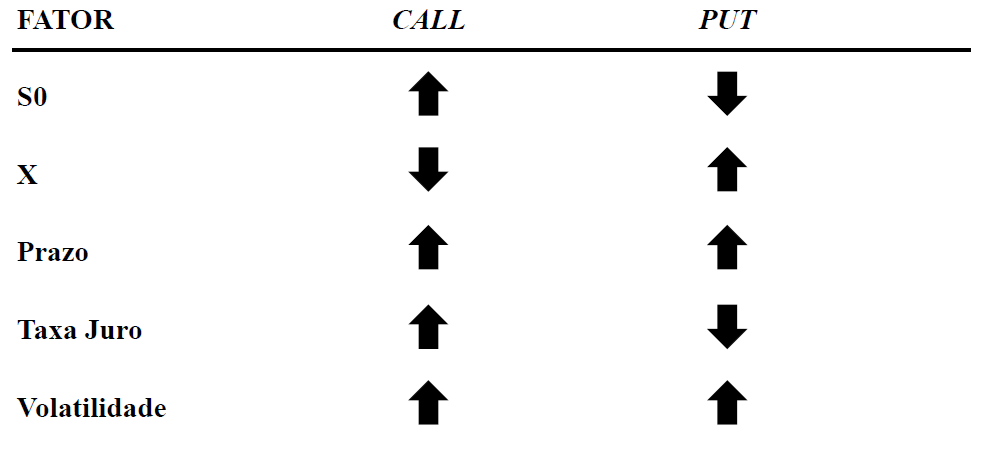
\includegraphics[width=1\linewidth]{image.png}
    \caption{Enter Caption}
    
\end{figure}
\section{Opções - Estratégias}
\subsection*{\textbf{Paridade Put-Call}}
\begin{center}\ovalbox{ \textbf{$\mathbf{p} + \mathbf{S_0} = \mathbf{c} + \mathbf{VP(X)}$} }
\end{center} 
É possível estimar os preços entre calls e puts por não arbitragem

\textbf{Válido para:}
\begin{itemize}
    \item Mesmo ativo objeto
    \item Mesmo vencimento
    \item Para calls e puts com o mesmo strike
\end{itemize}
\vspace{0.75 cm}
\subsection*{\textbf{Operações sintéticas com a paridade Put-Call}}
\begin{itemize}
    \item \textbf{Call:}  "Compro put + ação e tomo emprestado PV(X)"
    \begin{center}
    (Call) = P(Put) + P(Ação) - PV(X)  
    \end{center}
    \item \textbf{Put:} "compro uma call, vendo uma ação e aplico PV(X)"
    \begin{center}
P(Put) = P(Call) + PV(X) - P(Ação) 
    \end{center}
    \item \textbf{Ação:} "compro uma call, vendo uma put e aplico PV(X)"
    \begin{center}
P(Ação) = P(Call) + PV(X) - P(Put)  
    \end{center}
    \item \textbf{Título Rf:}"compro uma ação e uma put e vendo uma call"
    \begin{center}
PV(X) = P(Put) + P(Ação) - P(Call)
    \end{center}

\vspace{0.75 cm}
\subsection*{\textbf{Estratégias mais usuais}}
\item \textbf{Bull call spread:} compra de call com um preço de exercício (strike) mais baixo e venda de call com um preço de exercício (strike) mais alto 
\item \textbf{Bull put spread:} Venda de put com um preço de exercício (strike) mais alto e uma compra de put com um preço de exercício (strike) mais baixo.
\item \textbf{Bear call spread:} venda de call com um preço de exercício (strike) mais baixo e uma compra de call com um preço de exercício (strike) mais alto. 
\item \textbf{Bear Put spread:} compra de put com um preço de exercício (strike) mais alto e uma compra de put com um preço de exercício (strike) mais baixo. 
\item \textbf{Short butterfly spread with calls:} estratégia de 3 partes:

1. venda de call com strike mais baixo

2. compra de duas calls com strike mais alto 

3. venda de uma call com strike ainda mais alto. 
\item \textbf{Short condor spread with puts}: estratégia de 4 partes:

1. venda de uma put com um strike mais alto

2. compra de uma put com um strike mais baixo

3. compra de outra put com um strike ainda mais baixo 

4. venda de mais uma put com um strike ainda mais baixo


\section{\textbf{Apreçamento (Binomial e B\&S)}}
\subsection*{\textbf{Ideias iniciais}}

\end{itemize}

    \begin{center}
Call com prazo T, strike X, prêmio c em t = 0
    \end{center}
c = máx (S0 - X; 0) + \textbf{valor temporal}

\vspace{0.75 cm}
\textbf{Valor temporal:} mesmo que a call tenha valor intrínseco nulo hoje, o preço do ativo objeto pode subir o suficiente até o vencimento para superar o St.
\begin{itemize}
    \item Quanto maior a volatilidade do ativo objeto ou prazo de vendimento, maior será o valor temporal da call
\end{itemize}

\vspace{0.75 cm}
\subsection*{\textbf{Praticamente certo que não haverá exercio:}}
   \begin{center}
Caso  $S0 <<< X$ para a volatilidade ter efeito:
    \end{center}
\[\mathbf{c} \approx 0\]


       \begin{center}
Caso  $S0 >>> X$ para a volatilidade ter efeito:
    \end{center}


\[\mathbf{c} \approx \text{PV}(S_T - X) = S_0 - \text{PV}(D_T) - \text{PV}(X)\]

\vspace{0.75 cm}
\subsection*{\textbf{Determinantes do valor de calls e puts}}
\begin{figure}
    \centering
    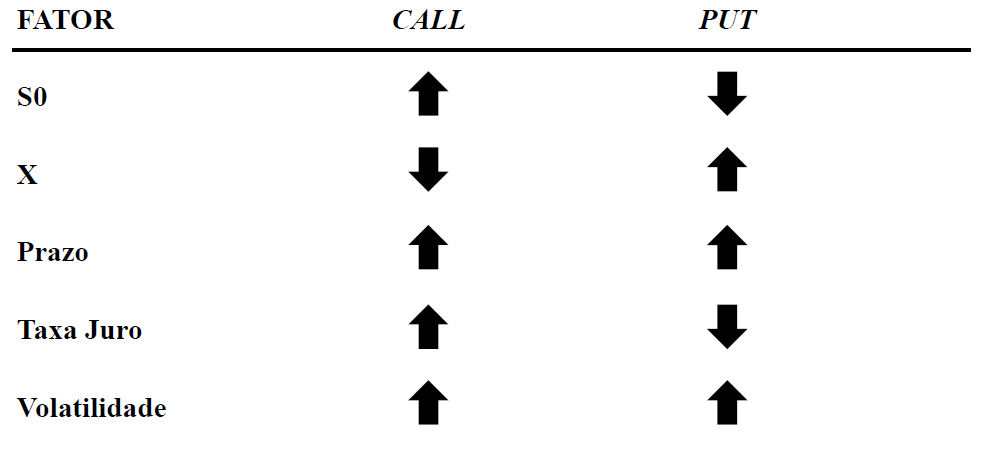
\includegraphics[width=0.5\linewidth]{image1.png}
    \caption{Enter Caption}
    \label{fig:enter-label}
\end{figure}

\end{multicols}

\end{document}
